\chapter{Frankenstein's Workshop: OOP Fundamentals}

\begin{figure}[h!]
    \centering
    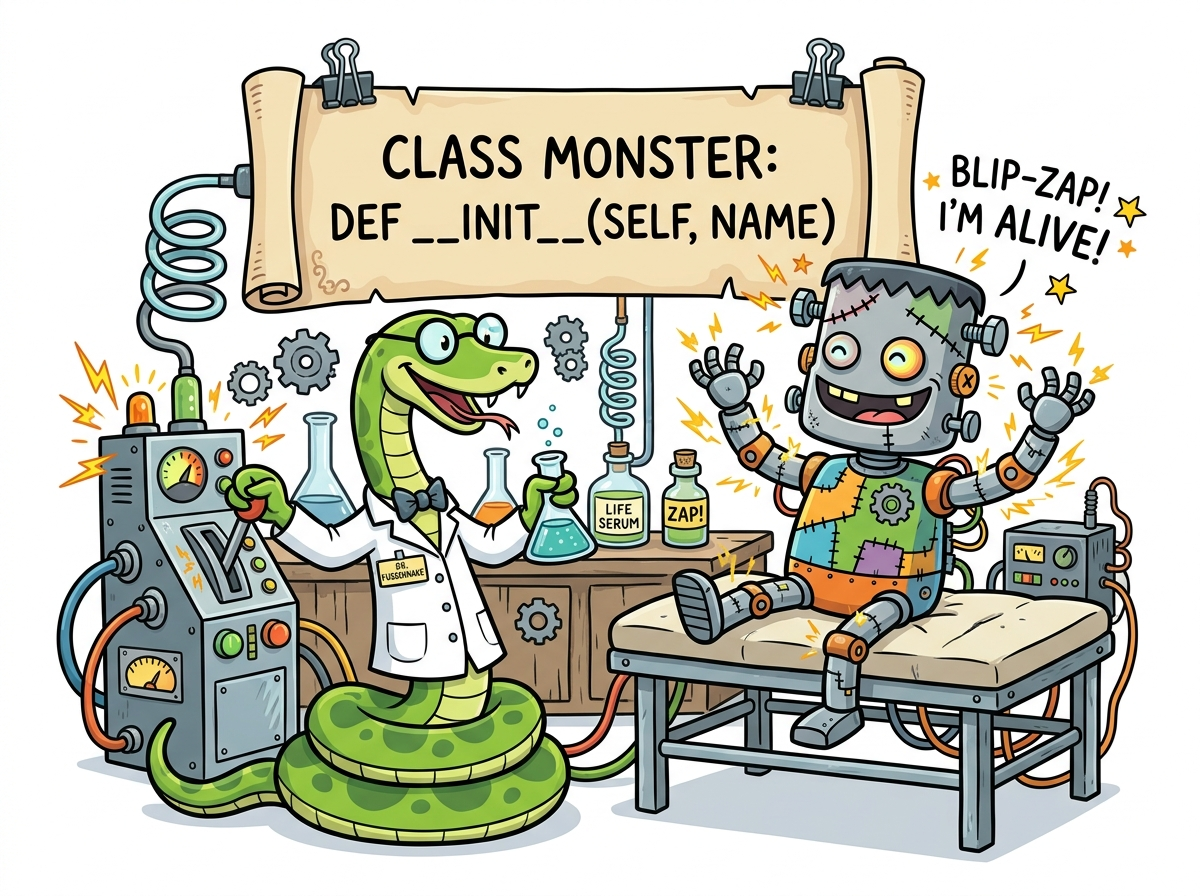
\includegraphics[width=0.75\textwidth]{images/ch7_monster_class.jpg}
    \caption{Classes are architectural blueprints; Objects are the living creations brought to life in memory!}
\end{figure}

\section{Thinking in Objects}

So far, we have treated data and functions as separate entities. But in the real world, things combine both! A car has data (\textit{color}, \textit{speed}) and actions (\textit{accelerate}, \textit{brake}).

\textbf{Object-Oriented Programming (OOP)} is a paradigm where we bundle related data (attributes) and functions (methods) into custom packages called \textbf{Objects}.

\section{Classes vs Objects: The Architectural Blueprint}

- \textbf{Class:} The blueprint or cookie cutter (e.g., \texttt{Monster}).
- \textbf{Object:} An actual instance baked using that cutter (e.g., \texttt{grumpy\_goblin}).

\begin{pycode}{Creating Your First Class}
class Monster:
    # Constructor method: runs when a new object is created
    def __init__(self, name, monster_type, hp):
        self.name = name            # Attribute
        self.monster_type = monster_type  # Attribute
        self.hp = hp                # Attribute

    # Method: Action the object can perform
    def roar(self):
        print(f"ROAR! {self.name} the {self.monster_type} threatens you with {self.hp} HP!")

# Instantiating objects from the class blueprint
goblin = Monster("Griznar", "Goblin", 45)
dragon = Monster("Ignis", "Fire Dragon", 500)

goblin.roar()
dragon.roar()
\end{pycode}

\section{Demystifying \texttt{self}}

Why does every method in a class take \texttt{self} as its first parameter?

Because \texttt{self} refers to the \textbf{specific object} currently calling the method! When \texttt{goblin.roar()} runs, \texttt{self} points to \texttt{goblin}. When \texttt{dragon.roar()} runs, \texttt{self} points to \texttt{dragon}.

\section{Inheritance: Passing Down the Family Genes}

You don't need to write every class from scratch! A child class can \textbf{inherit} attributes and methods from a parent class, and then add its own unique powers.

\begin{pycode}{Class Inheritance}
# Base Parent Class
class Hero:
    def __init__(self, name):
        self.name = name
        self.health = 100

    def rest(self):
        self.health += 20
        print(f"{self.name} rested. Health is now {self.health}.")

# Child Class inheriting from Hero
class Wizard(Hero):
    def __init__(self, name, mana):
        super().__init__(name) # Call Parent Constructor
        self.mana = mana

    def cast_spell(self):
        self.mana -= 10
        print(f"{self.name} cast a spell! Mana remaining: {self.mana}")

# Using the Wizard
merlin = Wizard("Merlin the Great", 100)
merlin.cast_spell()
merlin.rest() # Inherited from Hero parent class!
\end{pycode}

\section{Code Example: Bank Account Class with Encapsulation}

Here is a practical financial account class demonstrating data validation inside methods.

\begin{pycode}{BankAccount Class}
class BankAccount:
    def __init__(self, owner, initial_balance=0.0):
        self.owner = owner
        self.balance = initial_balance

    def deposit(self, amount):
        if amount > 0:
            self.balance += amount
            print(f"Deposited ${amount:.2f}. New Balance: ${self.balance:.2f}")

    def withdraw(self, amount):
        if 0 < amount <= self.balance:
            self.balance -= amount
            print(f"Withdrew ${amount:.2f}. Remaining Balance: ${self.balance:.2f}")
        else:
            print("Insufficient funds or invalid withdrawal amount!")

account = BankAccount("Alice", 100.00)
account.deposit(50.00)
account.withdraw(30.00)
\end{pycode}

\begin{snakesnack}{OOP Golden Rules}
1. Keep class names in \texttt{CamelCase} (e.g. \texttt{SpaceShip}, \texttt{UserProfile}).
2. Use attributes for *nouns* (data) and methods for *verbs* (actions).
3. Inheritance promotes code reuse, but don't over-engineer giant complex family trees!
\end{snakesnack}

\section{Practice Problems \& Exercises}

Bring your blueprints to life with these 3 OOP practice problems!

\begin{snakelab}{Problem 7.1: Car Mileage Tracker (Easy)}
Create a \texttt{Car} class with attributes \texttt{make}, \texttt{model}, and \texttt{odometer} (default $0$).
Add a method \texttt{drive(miles)} that increases \texttt{odometer} by \texttt{miles}.
Instantiate a car object, drive it twice, and print its odometer reading!
\end{snakelab}

\begin{pycode}{Solution 7.1: Car Mileage Tracker}
class Car:
    def __init__(self, make, model):
        self.make = make
        self.model = model
        self.odometer = 0

    def drive(self, miles):
        self.odometer += miles
        print(f"Drove {miles} miles. Odometer: {self.odometer} miles.")

my_car = Car("Cyber", "Truck")
my_car.drive(120)
my_car.drive(85)
\end{pycode}

\begin{snakelab}{Problem 7.2: Digital Shopping Cart (Medium)}
Create a \texttt{ShoppingCart} class:
\begin{itemize}
    \item Attribute: \texttt{items} (dictionary of item\_name -> price).
    \item Methods: \texttt{add\_item(name, price)}, \texttt{get\_total()}.
\end{itemize}
Instantiate a cart, add 3 items, and print the calculated total cost!
\end{snakelab}

\begin{pycode}{Solution 7.2: Digital Shopping Cart}
class ShoppingCart:
    def __init__(self):
        self.items = {}

    def add_item(self, name, price):
        self.items[name] = price

    def get_total(self):
        return sum(self.items.values())

cart = ShoppingCart()
cart.add_item("Python Book", 29.99)
cart.add_item("Coffee Mug", 12.50)
cart.add_item("Keyboard", 89.00)

print(f"Total Cart Value: ${cart.get_total():.2f}")
\end{pycode}

\begin{snakelab}{Problem 7.3: Employee \& Manager Hierarchy (Spicy)}
Create an \texttt{Employee} class with \texttt{name} and \texttt{salary}.
Create a child class \texttt{Manager(Employee)} with an additional attribute \texttt{department} and a method \texttt{hire\_bonus()} that increases their salary by \$5,000!
\end{snakelab}

\begin{pycode}{Solution 7.3: Employee Hierarchy}
class Employee:
    def __init__(self, name, salary):
        self.name = name
        self.salary = salary

class Manager(Employee):
    def __init__(self, name, salary, department):
        super().__init__(name, salary)
        self.department = department

    def hire_bonus(self):
        self.salary += 5000
        print(f"Manager {self.name} ({self.department}) received bonus! Salary: ${self.salary}")

boss = Manager("Sarah", 85000, "Engineering")
boss.hire_bonus()
\end{pycode}
